%\documentclass[11pt,dvipdfm]{article}
\documentclass[11pt,divpdfm]{article}
\usepackage{deauthor,times,graphicx}
\usepackage{marvosym}% for \Letter in author list
\usepackage{booktabs}% for \toprule, \midrule, \bottomrule in the table

%\graphicspath{{zhepeng/}}

\begin{document}
\title{BlockShare: A Blockchain Empowered System for Privacy-Preserving Verifiable Data Sharing}

\author{
Zhe Peng$^*$, Jianliang Xu$^*$\textsuperscript{(\Letter)}, Haibo Hu$^\dagger$, and Lei Chen$^\ddagger$\\
$^*$Hong Kong Baptist University\\
$^*$\{pengzhe, xujl\}@comp.hkbu.edu.hk\\
$^\dagger$Hong Kong Polytechnic University\\
$^\dagger$haibo.hu@polyu.edu.hk\\
$^\ddagger$Hong Kong University of Science and Technology\\
$^\ddagger$leichen@cse.ust.hk
}

% Corresponding author: Jianliang Xu.

\maketitle

\begin{abstract}
Data has become the most valuable resource, as it is essential to analytics, decision making, and artificial intelligence.
To unleash the value of data, data sharing has become a prerequisite to bringing tremendous benefits for both data providers and data consumers.
However, existing solutions for data sharing are mostly server-centric, i.e., they rely on the control of a trusted server, which increases security and privacy concerns among data users.
The design of a privacy-preserving verifiable data sharing framework to simultaneously secure user privacy and data integrity has not been sufficiently studied and remains a grand challenge.
In this paper, we propose BlockShare, a privacy-preserving verifiable data sharing system based on blockchain.
First, we design a novel blockchain-based architecture, together with a new authenticated data structure scheme to efficiently verify any portion of a shared data record in a decentralized fashion.
Second, we develop a zero-knowledge verification scheme that enables a user to prove a dynamic condition without disclosing the specific data attribute, minimizing privacy loss.
%maximally protecting data privacy.
We implement BlockShare and conduct experiments to evaluate the system performance.
Experimental results demonstrate the effectiveness of our proposed system.
\end{abstract}

\section{Introduction}
Data has been considered the ``oil" of the digital world, as it is essential to analytics, decision making, and artificial intelligence.
Recent years have witnessed increasing availability of personal data such as health, financial, and geo-social data.
Sharing such data with relevant stakeholders is a prerequisite for unleashing its value.
For example, sharing medical records with healthcare organizations can improve the quality of patient care, reduce insurance fraud, advance clinical research, and timely predict epidemic outbreaks like COVID-19.
To achieve secure data sharing, most existing systems rely on the security of cloud service providers, who claim to protect client data for storage and sharing.
%To unlock the value of data, data sharing is the key.

However, with the increasing value of data and growing cybersecurity threats, these cloud systems cannot fully address users' security and privacy concerns.
On the one hand, there have been many reported cloud security breaches, such as Apple's iCloud data leak in 2014 and Instagram's exposure of 49 million user accounts in 2019.
On the other hand, the Facebook-Cambridge Analytica data scandal in 2018 has exposed the issue of corporate dishonesty to grab users' data without consent for her benefit.
Both causes have affected users' willingness to share personal data using cloud-based solutions.
New data privacy legislation, such as the European Union General Data Protection Regulation (GDPR) \cite{gdpr} or the EFF's call for information fiduciary rules for businesses \cite{eff}, is an important step towards addressing data abuses, complemented by modern technological solutions that put users back into control.
% has reignited interest in secure management of private data.
% As a result, a recent survey by IBM has revealed that ``data silos", i.e., information isolation, is one of the greatest challenges for businesses and organizations of today.


Emerging blockchain or distributed ledger technology (DLT) has been adopted as a trustworthy data storage solution in various fields \cite{peng2021vfchain, peng2021p2b, wang2022vchain+}.
It allows trustless parties to collectively maintain a single version of data without a central authority.
By features of decentralization, immutability, and transparency, blockchain enables the decentralized and secure exchange of digital information and assets without a central trusted server.
As such, this new paradigm has fundamentally changed the way of data sharing and give rise to data markets controlled by users, instead of surrendering data governance to a few tech giants \cite{subramanian2017decentralized}.
It has also increased willingness to share data and break data silos to enforce cross-organization or even cross-border data cooperation.

From these observations, we identify the following key challenges that a secure blockchain empowered data sharing system should address.
First, \emph{data privacy} protection, especially during data storage and distribution, is known to have a critical impact on the uptake of such a system \cite{salman2018security}.
% data full life-cycle management
Therefore, concealing user privacy becomes the very first requirement in the full life cycle of data sharing.
Most current decentralized data sharing applications \cite{shen2019medchain, kang2018blockchain} utilize blockchain and smart contracts to accomplish the sharing of personal data.
However, existing approaches either forfeit availability guarantees for private data \cite{liang2017integrating} or fall back on semi-centralized solutions for key management \cite{cheng2020design, zyskind2015decentralizing}, thereby subduing data privacy to a single point of failure or compromise.
These potential system security issues might lead to serious private user data leakage.

Second, \emph{data integrity} verification is crucial to ensure the correctness of the data shared by blockchain.
This challenge is two-fold:
(i) how to securely and efficiently store data on the blockchain without incurring unaffordable storage and computational overheads;
and (ii) how to prevent data from being tampered with when sharing data with high granularity.
Prior systems \cite{matzutt2018quantitative, fan2018medblock, su2020lvbs} mainly adopt distributed ledger technology to store more general data and leverage smart contracts to control the data sharing process.
Nevertheless, since such general data (such as text, documents, and images) is usually large, it is not scalable to store raw data directly on-chain.
Even worse, most approaches are not capable of fine-grained data sharing to generate customized data records for various data consumers on-demand.
The integrity of a fragmented data record cannot be verified, which leaves space for data fraud.
% a fraction of data record, masked data record

To tackle the issues mentioned above, we propose BlockShare, a blockchain empowered data sharing system, which simultaneously secures user privacy and data integrity.
The system allows the data owner to dynamically generate data records for sharing with tailored privacy protection on an as-needed basis, where a trusted central server is unnecessary.
Concretely, we make the following contributions in the paper.
\begin{itemize}
	\item
	We introduce a novel BlockShare framework, together with a new \emph{authenticated data structure} scheme that can efficiently verify any portion of a shared data record in a decentralized fashion.
	\item
	We develop a \emph{zero-knowledge verification} scheme that enables a user to prove a dynamic condition without disclosing the specific data attribute, minimizing privacy loss.
	%maximally protecting data privacy.
	\item
	We implement BlockShare using readily-available infrastructural primitives.
	Experimental results show that our system achieves verifiable sharing of personal data in a privacy-preserving manner.
\end{itemize}



\section{Related Work}
In this section, we briefly review related studies and discuss relevant techniques.

\textbf{Blockchain and Smart Contract.}
Blockchain has recently raised major attention in both industries and academia, owing to the boom of cryptocurrencies such as Bitcoin \cite{nakamoto2008bitcoin}.
As a distributed and cryptographically hardened ledge, blockchain is recognized as a revolutionary technology for data-intensive applications.
Many new blockchain techniques, such as Ethereum \cite{Ethereum} and Hyperledger fabric \cite{androulaki2018hyperledger}, also introduce smart contracts to develop and execute customized programs on blockchain virtual machines.

In order to protect data privacy in blockchain systems, Kosba et al. \cite{kosba2016hawk} propose a framework for building privacy-preserving smart contracts.
The Hawk compiler could automatically compile the smart contract to a cryptographic protocol between contractual parties and the blockchain to retain transactional privacy.
Many researchers also devote their efforts to designing solutions to support various queries on the blockchain.
These methods, including VQL \cite{wu2021vql} and vChain \cite{xu2019vchain}, can help to greatly improve the query efficiency with data integrity guarantee for blockchain systems.
In addition, some approaches have been designed to efficiently store and manage blockchain data, such as SlimChain \cite{xu2021slimchain}, BlockchainDB \cite{el2019blockchaindb}, FalconDB \cite{peng2020falcondb}, and CALYPSO \cite{kokoris2020calypso}.
Due to the immutability and transparency features, we could build a secure and decentralized data sharing system based on blockchain.

\textbf{Blockchain-based Data Sharing.}
Data sharing has received extensive research attention with the advent of the big data era.
To keep data security and privacy in sharing, data is usually stored after encryption and further attached with certain access policies \cite{liu2012mona, pasquier2015camflow}.
In the traditional cloud setting, the centralized architecture is compromised with potential single-point failures or insider attacks \cite{wang2022privacy}.
Recently, many works have revealed some insights to show that the introduction of blockchain can significantly enhance system security in a decentralized way \cite{zheng2018scalable, qi2020cpds}.
Various applications have been developed for data sharing in healthcare, smart vehicles, IoT, and e-finance, using tokens as on-chain credentials for personal data \cite{yu2021blockchain, xia2017medshare}.

In addition to committing data records and recording sharing, blockchain can also provide functionalities such as access control, participant incentive, transaction auditing, and user identification for underlying data marketplaces, as well as providing services like dispute arbitration and data warranties for upper-layer data applications \cite{lu2020blockchain, shen2020blockchain}.
Many systems have been developed in recent years by leveraging blockchain and smart contracts to enhance data interoperability and unlock the economic benefits of data assets \cite{liu2018bpds}.

Nevertheless, given the unique properties that data can be replicated and redistributed, existing studies fail to address data privacy issues.
While many works adopt encryption of managed data records, a one-size-fits-all record often contains superfluous information, violating the ``minimum necessary" principle and creating privacy risks.



\section{System Overview}
In this section, we present the overview of our proposed BlockShare system for privacy-preserving verifiable data sharing.
% outline the architecture

\textbf{System Model.}
As illustrated in Figure \ref{fig:System}, the system model includes four parties: (i) \emph{data source}, (ii) \emph{data owner}, (iii) \emph{blockchain}, and (iv) \emph{data consumer}.
% data provider
To protect data privacy and make the whole system scalable, a decentralized storage architecture is employed.
Specifically, raw data from various sources (e.g., health records, financial transactions, and social contacts) are generated and stored off-chain by their data owners (i.e., users).
Each data object is modeled as a tuple $o_i = <id, V_i>$, where $id$ denotes the object's ID, and $V_i$ defines a set of data attributes.
Meanwhile, an \emph{authenticated data structure} (ADS) will be constructed for each data record and stored on the blockchain.
The on-chain ADSs are immutable, serving as notarizations of the raw data.

In order to unlock the value of data, the data owner can prepare tailored data records with different privacy protection levels and share them with relevant stakeholders.
For example, a vaccine certificate (or ``vaccine passport") with only the coarse-grained vaccination information is issued when entering restaurants, while a vaccine passport with detailed vaccination and personal information will be made for use at the customs.
After receiving the shared data record, the data consumer (e.g., hospital, customs, or insurance company) verifies the data integrity without violating the user's privacy.
% with privacy concerns.
On the one hand, the integrity of the data record is checked with the corresponding ADS obtained from the blockchain such that no fraudulent data is transmitted.
On the other hand, the data owner can generate a zero-knowledge proof for the data consumer such that personal information disclosure can be controlled with high granularity.


\textbf{Threat Model.}
In our system, security threats come from two aspects:
(i) the data owner is not fully trusted and might modify the requested data records intentionally or unintentionally;
and (ii) the data consumer is curious and may attempt to infer some knowledge pertaining to its interests from the received data.
To address these threats, we need to ensure data integrity without compromising users' privacy during data sharing.
Concretely, we define three criteria of security constraints as follows:
% properties
\begin{itemize}
	\item
	\textbf{Soundness.} All of the shared data records are not tampered with and are truly the results with respect to the data consumer's desires.
	% are originated from the data source.
	This is a basic requirement for any data sharing service.
	\item
	\textbf{Completeness.} No valid data attributes are missing regarding the data sharing request.
	That is, the shared data record is complete during the process of fine-grained data sharing.
	\item
	\textbf{Zero-Knowledge Confidentiality.}
	Any information beyond the ``minimum necessary" standard is protected.
	That is, the data owner can prove a data attribute satisfying a specific condition without disclosing the concrete attribute value or even its size.
\end{itemize}

In addition, we assume that there is no collusion between data sources, data owners, and data consumers.
Regarding the blockchain, we also assume that the adversary cannot gain any advantage in attacking the consensus protocol and thus the execution integrity of the smart contract is guaranteed.

\begin{figure}[t]
	\centering
	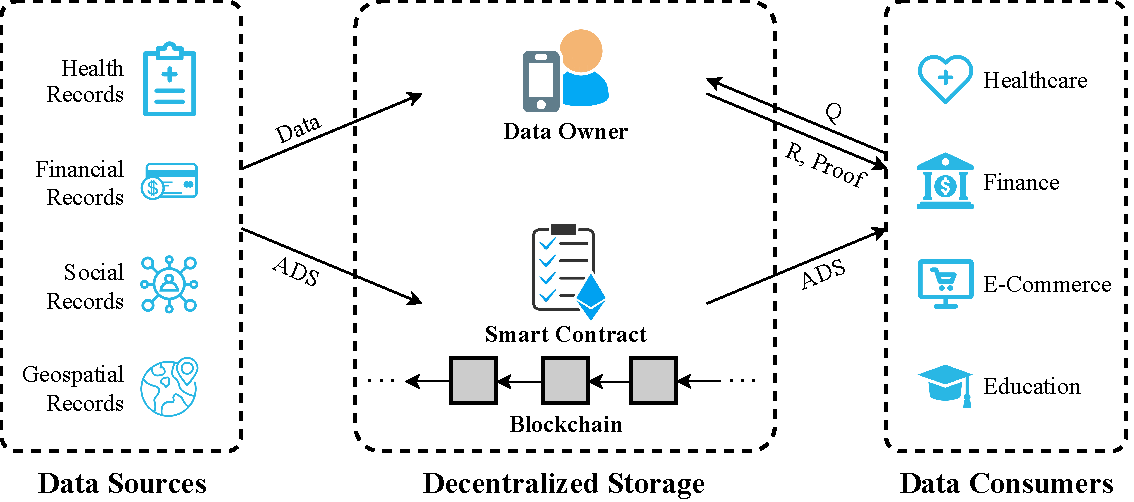
\includegraphics[width=0.9\textwidth]{figs/Fig_System.pdf}
	\caption{System Model of BlockShare}
	\label{fig:System}
\end{figure}


\section{BlockShare Design}
In this section, we present BlockShare, a privacy-preserving and verifiable data sharing initiative based on blockchain.
We begin by introducing a dynamic data verification scheme to efficiently verify multiple versions of the shared data record with high granularity.
Furthermore, we propose a zero-knowledge condition verification scheme to maximally protect the privacy of personal data under the umbrella of data integrity.

\subsection{Dynamic Data Verification}
\textbf{ADS Construction and Storage.}
The verification for the shared data is built upon a blockchain-based decentralized storage model.
Recall that in the proposed BlockShare architecture, original data records are generated from the trusted data sources and distributed to the relevant data owners for local storage.
At the same time, an authenticated data structure (ADS) is constructed for each data record and kept on-chain as a proof of data integrity.
Concretely, we utilize Merkle Hash Tree (MHT) \cite{merkle1989certified} to derive a Merkle Root (serving as the ADS) to support data integrity verification.

We use Figure \ref{fig:ADS} as an example to show the ADS construction of the COVID-19 vaccination record.
In view of the surge of COVID-19 cases in the community, many countries have developed an immunization information system to manage vaccination records for pandemic control.
Generally, the vaccination record consists of three parts, including personal information, vaccination information, and testing information (e.g., nucleic acid test and serum IgG antibody test).
In order to prove the virus immunity, citizens are required to show their vaccine passports when entering some premises.
During this process, one challenge is that the user might forge or modify historical vaccination records to generate a fake vaccine passport for some purposes (e.g., avoiding quarantine, extending the expiration date of vaccination, or protecting privacy).
% obtaining privilege

To remedy this problem, we build a semantic-oriented MHT to accurately model each part of the vaccination record.
Specifically, to enhance data privacy and prevent rainbow attacks, a unique random number will be
associated with each attribute in the data record to generate a ``salted" record.
As such, each leaf node contains a hash value $h_{leaf}$ computed as
$h_{leaf} = H(H(v) \| H(nonce))$,
where $H(\cdot)$ is a cryptographic hash function, $v$ is the value of attribute, $nonce$ is an attribute-specific random number, and ``$\|$" denotes the concatenation operation.
The hash value stored on each internal node is recursively calculated using its all child nodes.
Finally, as illustrated in Figure \ref{fig:ADS}, the Merkle Root is generated on the top of three independent sub-trees.

In addition, as the write operation on the blockchain is very extensive, the frequent on-chain storage of the whole MHT would incur massive gas consumption.
At the same time, we observe that only the Merkle Root is needed from the blockchain during the data authentication.
Therefore, an optimal method is to suppress all nodes in the MHT and only materialize the Merkle Root on the blockchain.



\begin{figure*}[t]
	\centering
	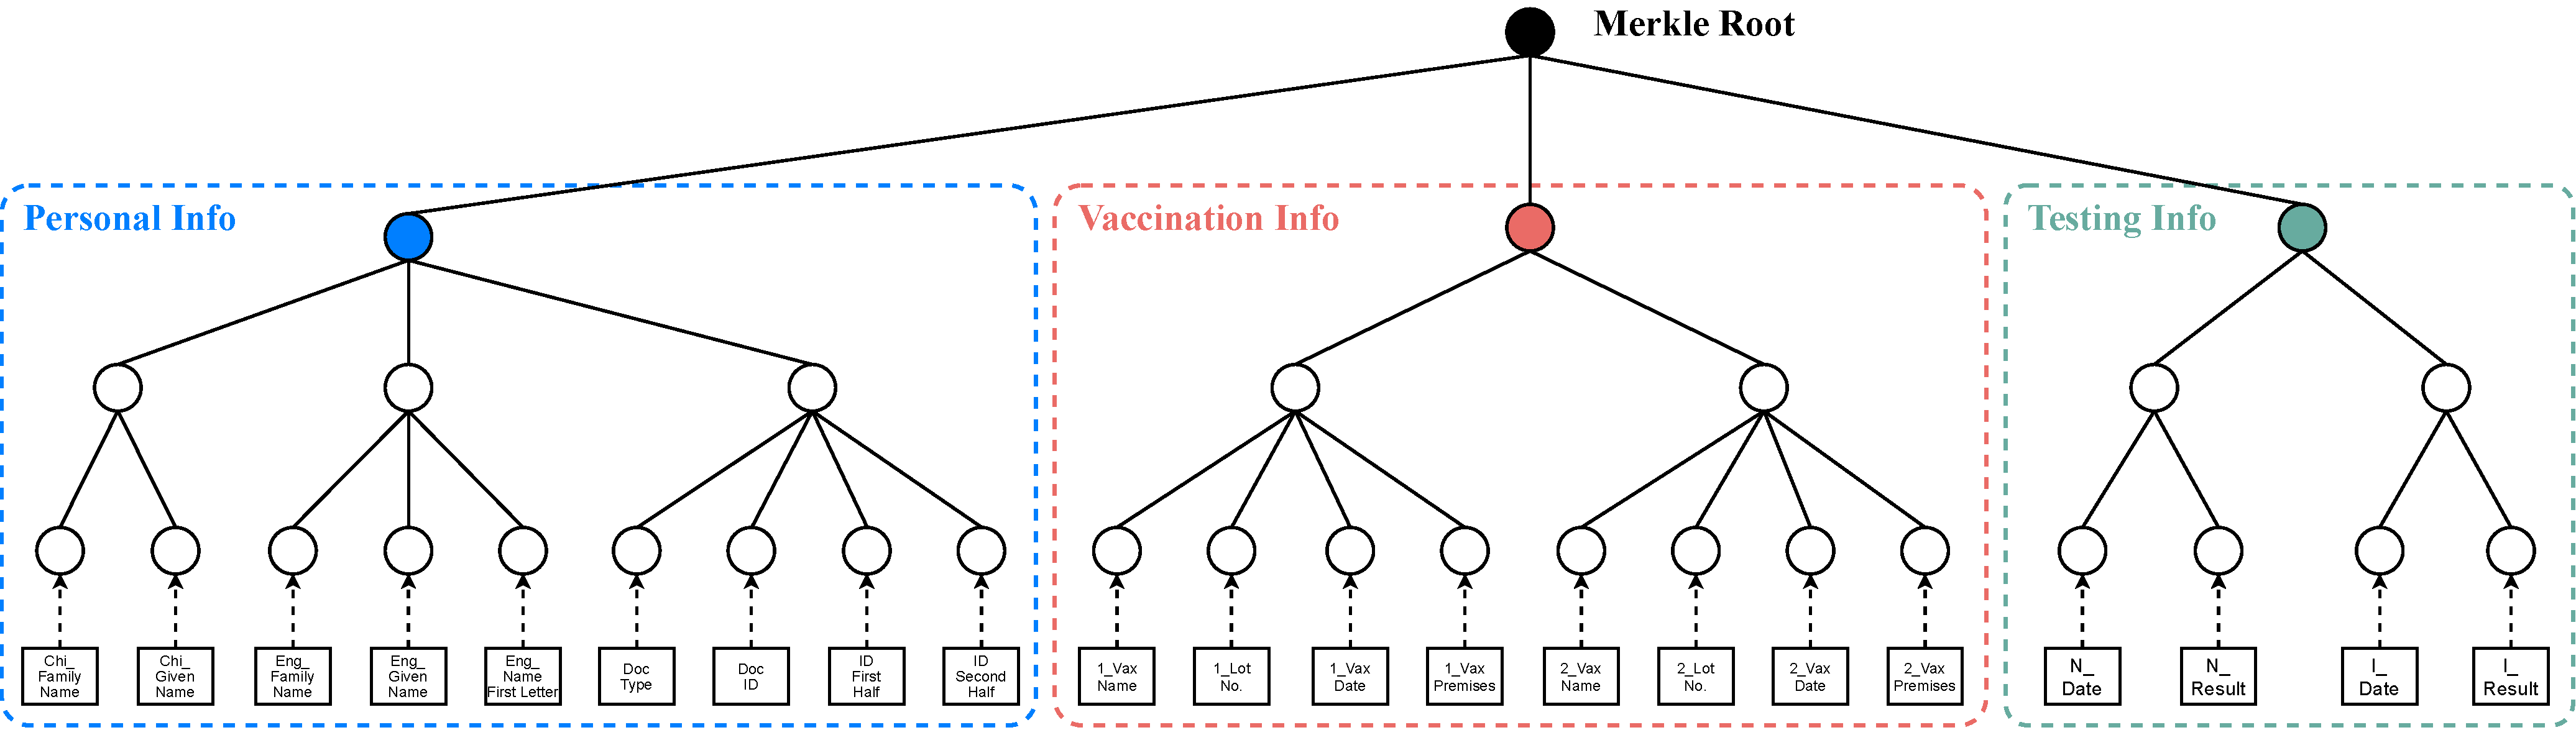
\includegraphics[width=0.9\textwidth]{figs/Fig_ADS.pdf}
	\caption{ADS Construction Example for the Vaccination Record}
	\label{fig:ADS}
\end{figure*}

\textbf{Information Masking and Verification.}
In practical data sharing, the diversity of privacy protection levels exists in many scenarios.
The data owner might prefer to issue a tailored data record by sharing a portion of data attributes according to the dynamic requirements.
For instance, the user can only indicate whether he/she has been vaccinated during a period without disclosing the entire ID number, vaccine name, vaccine lot number, and vaccination premises.
It would be costly, if not impossible, to generate and store a specialized ADS for each version of the data record.
As such, we propose a new ``one-ADS-for-multiple-versions" paradigm in which the data source only needs to generate a single ADS for one data record and store the ADS on the blockchain.

More specifically, for a given attribute in a data record, many sub-attributes will be appended in the MHT as leaf nodes to support different privacy constraints.
For example, as shown in Figure \ref{fig:ADS}, two more sub-attributes (i.e., the first half of ID and the second half of ID) are derived from the ID number and added to the MHT.
With this appended MHT, the data owner has multiple options to disclose the concrete content in the data record, while the Merkle Root keeps unique for verification.
Furthermore, the data owner can mask unnecessary attributes into hash values to generate a specific version of the data record.
For the shared attributes in the data record, the data owner generates a verification object (i.e., the Merkle Path) based on the unique ADS.
Then, with the verification object and the on-chain ADS, the data consumer can verify the integrity of the received data record (e.g., the tailored vaccine passport).

\subsection{Zero-Knowledge Privacy Protection}
In the previous information masking scheme, although the unnecessary attributes can be masked to protect privacy, the shared data attributes might still contain more personal information than what is needed.
For example, to show that the vaccination has been completed for a period (e.g., 14 days), the campus visitor has to disclose the concrete vaccination date.
Thus, to further enhance privacy, we propose a general privacy protection scheme for the shared data attributes based on non-interactive zero-knowledge (NIZK) proof technology \cite{bootle2016efficient}.
This scheme enables the data owner to prove a dynamic condition without revealing the specific value, limiting the disclosure of personal data to the minimum necessary while guaranteeing data integrity.

In this scheme, a constraint will be first defined for a specific attribute.
Usually, this constraint represents the data information needed by the data consumer.
Then, the data owner will generate a proof of satisfiability and pass it without the attribute value to the data consumer for verification.
With this scheme, the data owner can indicate only a qualified period instead of a detailed date, an area instead of a concrete vaccination premise, or an age group instead of exact age.
Given a constraint of an attribute, we present the formal definition of the zero-knowledge condition verification as follows:


\begin{definition}[Zero-Knowledge Condition Verification]
	For the input attribute value $v$, a range $R$, a random number $nonce$ associated with the attribute, the hash value $h$ of the attribute, ADS $mRoot$ of the data record $o$, and global parameters $G, H \in E(F_q)$, this scheme can prove to a verifier that the prover knows an assignment to $v$ such that $hash(v, nonce)=h ~ \wedge ~ v \in R$, without revealing $v$.
	It consists of the following algorithms:
	\begin{itemize}
		\item
		$\{\textbf{G}=(G_1, \cdots, G_n), \textbf{H}=(H_1, \cdots, H_n), G, H\} \leftarrow \textsf{Setup}(1^ \lambda)$:
		Call the parameter generation algorithm $\textsf{Setup}$ to generate public security parameters for zero-knowledge proof.
		On input a security parameter $1^ \lambda$, it outputs public parameters $\{\textbf{G}, \textbf{H}, G, H\}$ acting as implicit input for other functions.
		
		\item
		$\pi \leftarrow \textsf{zkProofGen}(v, nonce, R, h)$:
		The prover calls the zero-knowledge proof generation algorithm $\textsf{zkProofGen}$ to generate a proof for the shared attribute with zero knowledge.
		On input an attribute value $v$, the random number $nonce$ associated with the attribute, a range $R$ for the attribute, and the hash value $h$ of the corresponding leaf node, it outputs a zero-knowledge proof $\pi$.
		
		\item
		$mPath \leftarrow \textsf{mkProofGen}(h, mTree)$:
		The prover calls the Merkle proof generation algorithm $\textsf{mkProofGen}$ to generate a proof
		for the leaf node with the Merkle tree.
		On input the hash value $h$ of the corresponding leaf node, and a Merkle tree $mTree$, it outputs a Merkle path $mPath$.
		
		\item
		$\{0, 1\} \leftarrow \textsf{zkProofVer}(\pi, R, h)$:
		The verifier calls the zero-knowledge proof verification algorithm $\textsf{zkProofVer}$ to verify
		the received zero-knowledge proof.
		On input a zero-knowledge proof $\pi$, a range $R$ for the attribute, and the hash value $h$ of the corresponding leaf node, it outputs 1 if the verification is valid.
		
		\item
		$\{0, 1\} \leftarrow \textsf{mkProofVer}(h, mPath, mRoot)$:
		The verifier calls the Merkle tree authentication algorithm \textsf{mkProofVer} to verify the received Merkle proof.
		On input the hash value $h$ of the corresponding leaf node, the received Merkle path $mPath$, and the public Merkle root $mRoot$, it outputs 1 if the verification is valid.
	\end{itemize}
\end{definition}


To summarize, owing to the dynamic data verification and zero-knowledge proof design, the data sharing process is verifiable while the data owner has full control over the information disclosure through the following features:
\begin{itemize}
	\item \textbf{Multi-version support.}
	The data owner can dynamically generate multiple versions of a data record to meet different application needs.
	\item \textbf{Data integrity support.}
	The data owner can support integrity verification for multiple versions of a data record by using a single ADS.
	\item \textbf{Privacy protection support.}
	The data owner can quantify the information disclosure with different privacy protection levels using two predominant privacy metrics:
	(i) \emph{Suppression}: the data owner can mask partial information of a data record with high granularity, while an adversary is unable to infer the preimage of the masked information.
	(ii) \emph{Generalization}: a shared data attribute can be generalized to an arbitrary coarse granularity, for example, ``more than 2 weeks" instead of a concrete date and ``in the 20-30 age group" instead of exact age.
\end{itemize}




\section{Implementations and Evaluation}
In this section, we present the implementation of BlockShare and evaluate its performance in detail.

\subsection{Experimental Implementation}
We have designed and implemented a prototype of BlockShare, including the data source, data owner, and data consumer in JavaScript and Python, and the blockchain in Solidity.
Arithmetic circuits for NIZK proofs, along with the core logic of circuit compilation, universal setup, proof generation and verification are implemented using Circom and Snarkjs.
We perform the evaluation on a desktop computer with a 3.6 GHz Intel Xeon processor, 64 GB RAM, and 1 TB SSD.
All experiments are conducted based on a synthetic dataset.




\subsection{Performance Evaluation}
\emph{1) ADS Construction:}
We first perform an evaluation on the time cost of ADS generation at three length settings of hash functions based on the data records of 1K, 2K, 4K, 8K, and 16K entries, respectively.
As we can see from Figure \ref{fig:ResultADS}, the time cost of ADS construction raises linearly in all cases as the amount increases.
It only takes roughly 74ms to construct ADSs for 1K records and 0.8s for all of 16K records, when the hash value has 128 bits.
In addition, although calculating a longer hash value usually needs more time, constructing ADSs with 512-bit length for all of 1K records can still be finished in 0.2s.
When the amount of records increases to 16K, only 3s will be needed to finish the ADS construction process.
These benefits come from the high efficiency of a hash function.



\begin{figure*}[t]
	\centering %图片全局居中
	%并排几个图,就要写几个minipage
	\begin{minipage}[b]{0.4\textwidth} %所有minipage宽度之和要小于1,否则会自动变成竖排
		\centering %图片局部居中
		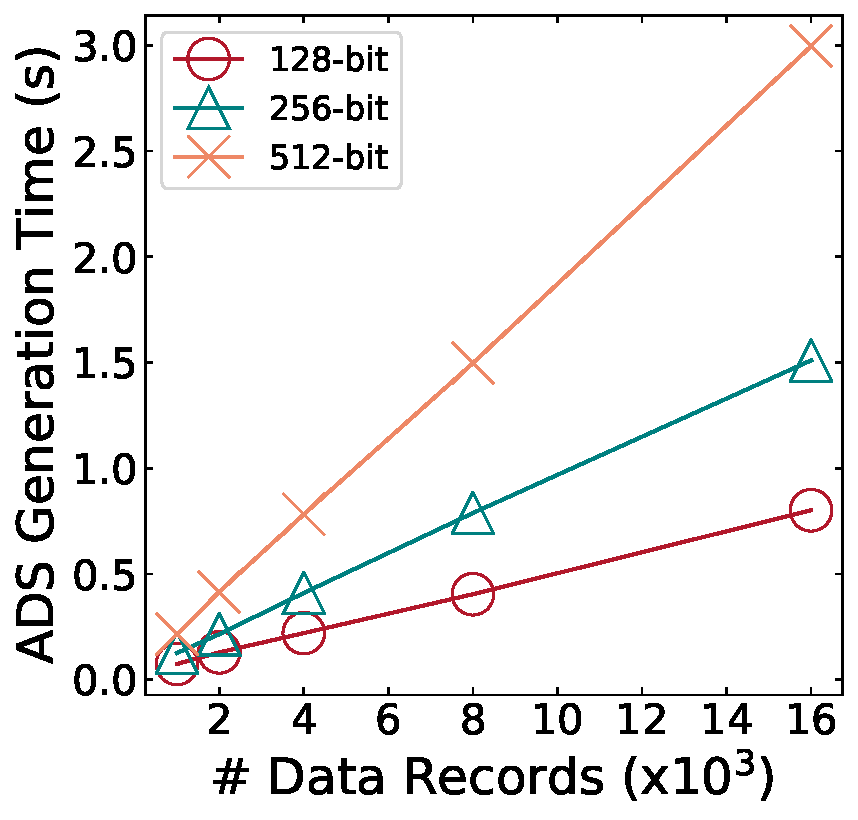
\includegraphics[width=1\textwidth]{figs/Result_ADS.pdf} %此时的图片宽度比例是相对于这个minipage的,不是全局
		\caption{Time cost of ADS generation}
		\label{fig:ResultADS}
	\end{minipage}
	\begin{minipage}[b]{0.4\textwidth} %所有minipage宽度之和要小于1,否则会自动变成竖排
		\centering %图片局部居中
		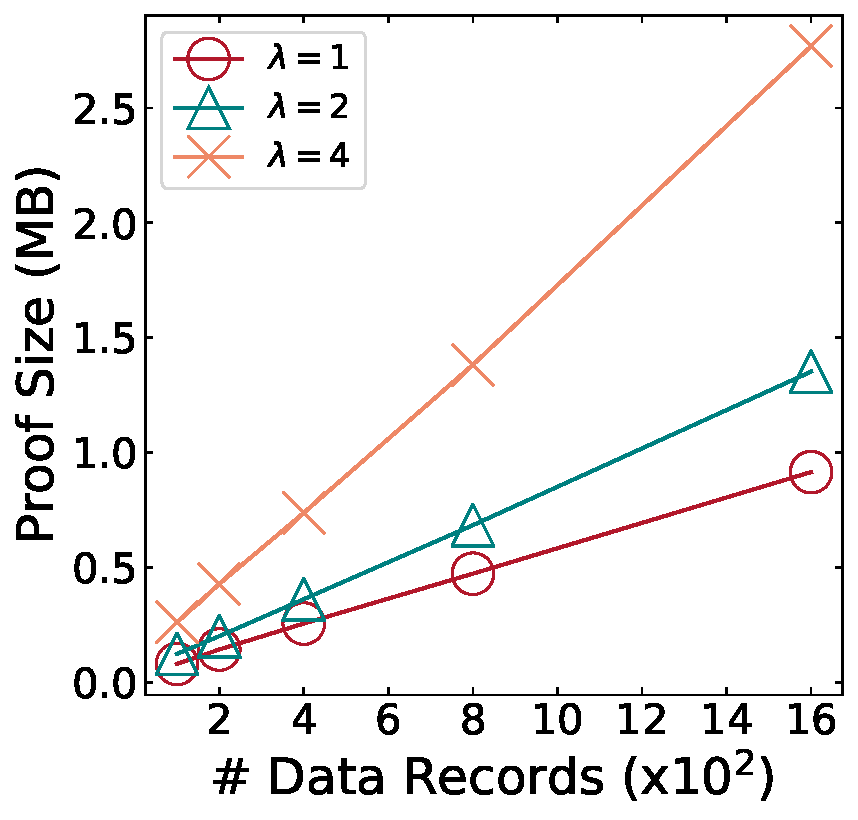
\includegraphics[width=1\textwidth]{figs/Result_ProofSize.pdf}%此时的图片宽度比例是相对于这个minipage的,不是全局
		\caption{Storage cost of NIZK proof}
		\label{fig:ResultProofSize}
	\end{minipage}
	%\vspace{-1em}
\end{figure*}

\begin{figure*}[t]
	\centering %图片全局居中
	%并排几个图,就要写几个minipage
	\begin{minipage}[b]{0.4\textwidth} %所有minipage宽度之和要小于1,否则会自动变成竖排
		\centering %图片局部居中
		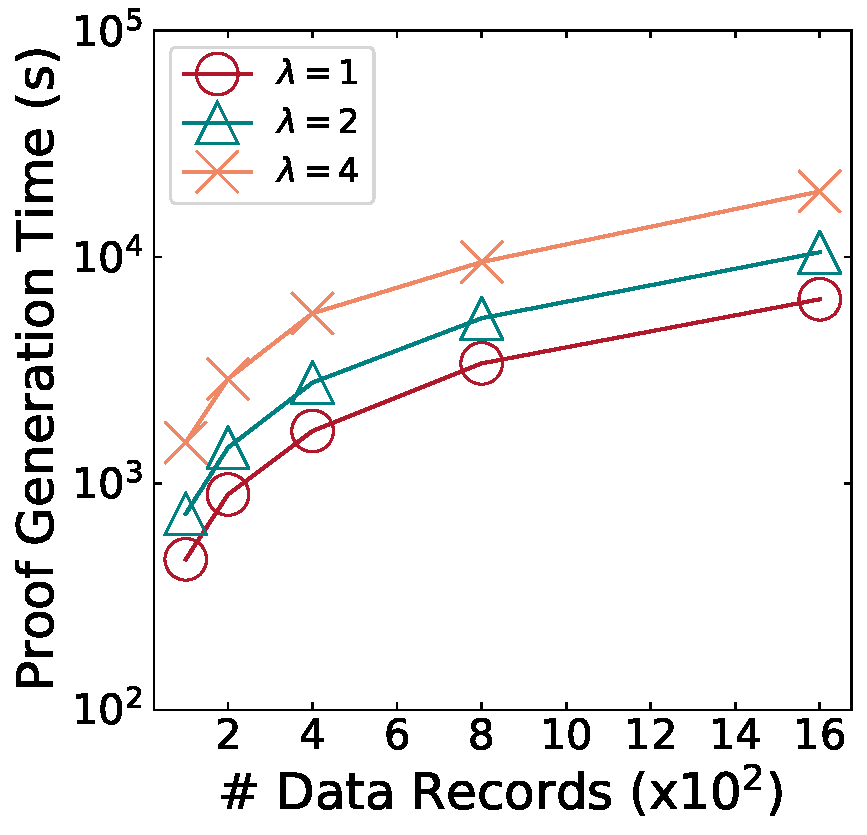
\includegraphics[width=1\textwidth]{figs/Result_ProverTime.pdf} %此时的图片宽度比例是相对于这个minipage的,不是全局
		\caption{Time cost of proof generation}
		\label{fig:ResultProverTime}
	\end{minipage}
	\begin{minipage}[b]{0.4\textwidth} %所有minipage宽度之和要小于1,否则会自动变成竖排
		\centering %图片局部居中
		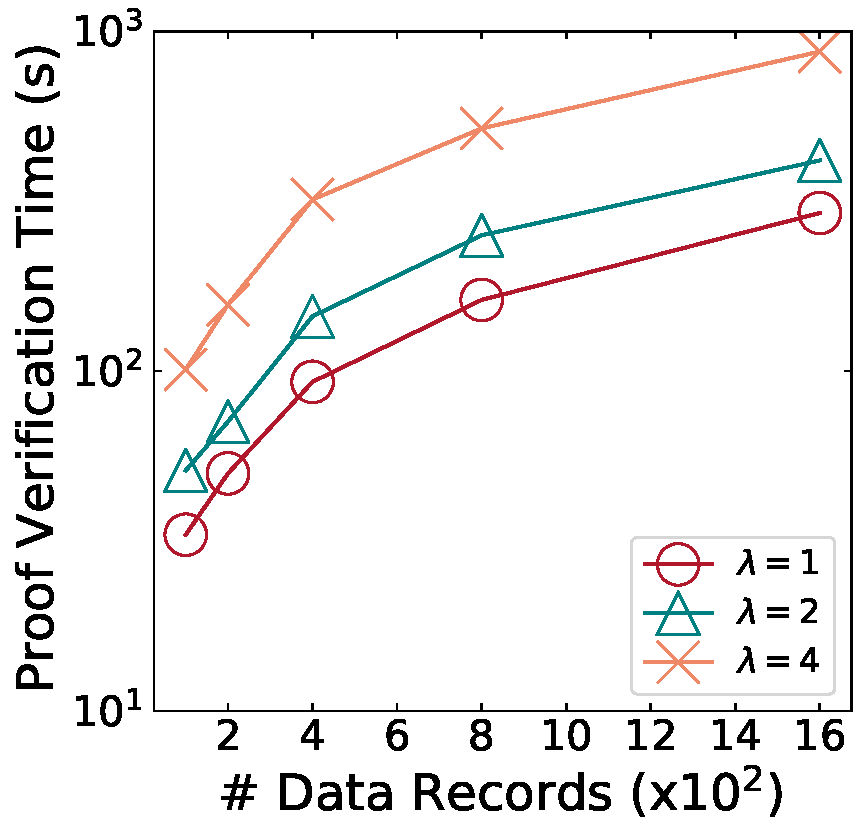
\includegraphics[width=1\textwidth]{figs/Result_VerifierTime.pdf} %此时的图片宽度比例是相对于这个minipage的,不是全局
		\caption{Time cost of proof verification}
		\label{fig:ResultVerifierTime}
	\end{minipage}
	%\vspace{-1em}
\end{figure*}


\emph{2) Proof Performance:}
We further evaluate the zero-knowledge verification scheme with three metrics: (i) NIZK proof size, (ii) proof generation time, and (iii) proof verification time.
We use $\lambda$ to indicate how many conditions need to be proved for corresponding attributes in a data record.
For each metric, three comparison experiments are conducted, with different values of $\lambda$, including 1, 2, and 4, respectively.

Figure \ref{fig:ResultProofSize} shows the total size of NIZK proofs when the number of data records is varied from 100 to 1.6K.
Our proposed scheme needs 80KB of storage space, if there are 100 data records and each record has one condition to be proved.
Moreover, if we increase the dataset volume to 1.6K and each record has four conditions to be proved, the total storage cost for the proofs is limited to 2.7MB.
It can be concluded that the proof size keeps succinct ($< 3$ MB) in BlockShare.

Figure \ref{fig:ResultProverTime} illustrates the total proof generation cost in terms of prover CPU time with a varied amount of data records.
For a dataset consisting of 100 records, it takes about 7 minutes to complete the proof generation for all records when each record has an attribute to be protected with zero-knowledge privacy.
We can find that the increase in proof generation time is noteworthy with the raising of dataset size and constraint volume.
The reason is that our implementation of zero-knowledge condition verification based on arithmetic circuits trades the proof generation time for a succinct proof size to save communication bandwidth.
To ease this issue, a potential method is to pre-generate and re-use the proof for a specific condition.

In Figure \ref{fig:ResultVerifierTime}, we plot the total proof verification cost in terms of verifier CPU time with regard to the number of data records.
The proof verification process could be completed in only 33s when there are 100 data records and one condition for each record.
If we increase the number of records to 1.6K, 5 minutes will be spent to verify all of the data records.
Compared with the proof generation process, we can see that our zero-knowledge proof verification is more efficient.
High verification efficiency could be an advantage to encourage more data consumers to join the data sharing system.



\emph{3) Gas Consumption:}
The smart contract in BlockShare is deployed on the Goerli testnet of Ethereum, enforcing the storage and request of ADS on the blockchain.
As shown in Table \ref{tab:Gas}, the deployment is a one-time effort, costing approximately 530,548 gas.
Gas spent for method invocation is also evaluated.
Since ADSs only record and manage the metadata of data records, the gas spent for the ADS storage function is quite economical.
It only costs 69,923 gas per time for the 256-bit ADS regardless of the size of a data record.
Regarding the gas of the on-chain ADS request for data verification, it costs around 29,402 gas, i.e., approximately $\$$0.06 when ETH is at the price of $\$$2,000.
The gas appears practically low because reading a value on the blockchain is very cheap in gas.



\begin{table}[h]
	\caption{Gas consumption of smart contract}
	\label{tab:Gas}
	\centering
	\setlength{\tabcolsep}{7mm}{
		\begin{tabular}{cc}
			\toprule
			\textbf{Operation} & \textbf{Gas Consumed} \\
			\midrule
			Contract Deployment  & 530,548 \\
			ADS Storage  & 69,923 \\
			ADS Request  & 29,402 \\
			\bottomrule
		\end{tabular}
	}
	%\vspace{-1em}
\end{table}






\section{Conclusion}
In this paper, we propose BlockShare, a privacy-preserving verifiable data sharing system based on blockchain.
We first design a novel blockchain-based decentralized architecture, together with a new authenticated data structure scheme to efficiently verify any portion of a shared data record.
Then, we develop a zero-knowledge verification scheme allowing a user to prove a dynamic condition without disclosing the specific data attribute, maximally protecting data privacy.
We implement BlockShare and experimental results show that our system achieves verifiable sharing of personal data in a privacy-preserving manner.


\section*{Acknowledgement}
This work was supported by Hong Kong RGC Grants C2004-21GF, 12202221, and 12201520.



%\bibliographystyle{ieeetr}
%\bibliography{exbible}


%\begin{thebibliography}{10}
%	\itemsep=1pt
%	\begin{small}
%		
%		\bibitem{askit2012} R.~Boim, O.~Greenshpan, T.~Milo, S.~Novgorodov, N.~Polyzotis, and W.-C. Tan. \newblock Asking the right questions in crowd data sourcing. \newblock {\em ICDE}, 0:1261–1264, 2012.
%		
%		\bibitem{peng2021p2b} Z. Peng, C. Xu, H. Wang, J. Huang, J. Xu, and X. Chu. \newblock {P2B-Trace: Privacy-preserving blockchain-based contact tracing to combat pandemics.} In \newblock {\em Proceedings of the ACM international conference on management of data (SIGMOD)}, 2021.
%		
%		
%	\end{small}
%\end{thebibliography}


\begin{thebibliography}{10}

\bibitem{gdpr}
{European Parliament and Council of the European Union}, ``{General Data
  Protection Regulation (GDPR)},'' {\em Official Journal of the European Union
  (OJ) L119}, pp.~1--88, 2016.

\bibitem{eff}
A.~Schwartz and C.~Cohn, ``{``Information Fiduciaries" Must Protect Your Data
  Privacy},'' {\em Electronic Frontier Foundation}, 2018.

\bibitem{peng2021vfchain}
Z.~Peng, J.~Xu, X.~Chu, S.~Gao, Y.~Yao, R.~Gu, and Y.~Tang, ``{VFChain}:
  enabling verifiable and auditable federated learning via blockchain
  systems,'' {\em IEEE Transactions on Network Science and Engineering},
  vol.~9, no.~1, pp.~173--186, 2021.

\bibitem{peng2021p2b}
Z.~Peng, C.~Xu, H.~Wang, J.~Huang, J.~Xu, and X.~Chu, ``{P$^2$B-Trace}:
  Privacy-preserving blockchain-based contact tracing to combat pandemics,'' in
  {\em Proc. of ACM SIGMOD International Conference on Management of Data},
  2021.

\bibitem{wang2022vchain+}
H.~Wang, C.~Xu, C.~Zhang, J.~Xu, Z.~Peng, and J.~Pei, ``{vChain+}: Optimizing
  verifiable blockchain boolean range queries,'' in {\em Proc. of IEEE
  International Conference on Data Engineering (ICDE)}, 2022.

\bibitem{subramanian2017decentralized}
H.~Subramanian, ``Decentralized blockchain-based electronic marketplaces,''
  {\em Communications of the ACM}, vol.~61, no.~1, pp.~78--84, 2017.

\bibitem{salman2018security}
T.~Salman, M.~Zolanvari, A.~Erbad, R.~Jain, and M.~Samaka, ``Security services
  using blockchains: A state of the art survey,'' {\em IEEE Communications
  Surveys \& Tutorials}, vol.~21, no.~1, pp.~858--880, 2018.

\bibitem{shen2019medchain}
B.~Shen, J.~Guo, and Y.~Yang, ``{MedChain}: Efficient healthcare data sharing
  via blockchain,'' {\em Applied Sciences}, vol.~9, no.~6, pp.~1--23, 2019.

\bibitem{kang2018blockchain}
J.~Kang, R.~Yu, X.~Huang, M.~Wu, S.~Maharjan, S.~Xie, and Y.~Zhang,
  ``Blockchain for secure and efficient data sharing in vehicular edge
  computing and networks,'' {\em IEEE Internet of Things Journal}, vol.~6,
  no.~3, pp.~4660--4670, 2018.

\bibitem{liang2017integrating}
X.~Liang, J.~Zhao, S.~Shetty, J.~Liu, and D.~Li, ``Integrating blockchain for
  data sharing and collaboration in mobile healthcare applications,'' in {\em
  Proc. of IEEE international symposium on personal, indoor, and mobile radio
  communications}, pp.~1--5, 2017.

\bibitem{cheng2020design}
X.~Cheng, F.~Chen, D.~Xie, H.~Sun, and C.~Huang, ``Design of a secure medical
  data sharing scheme based on blockchain,'' {\em Journal of medical systems},
  vol.~44, no.~2, pp.~1--11, 2020.

\bibitem{zyskind2015decentralizing}
G.~Zyskind, O.~Nathan, {\em et~al.}, ``Decentralizing privacy: Using blockchain
  to protect personal data,'' in {\em Proc. of IEEE Security and Privacy
  Workshops}, 2015.

\bibitem{matzutt2018quantitative}
R.~Matzutt, J.~Hiller, M.~Henze, J.~H. Ziegeldorf, D.~M{\"u}llmann,
  O.~Hohlfeld, and K.~Wehrle, ``A quantitative analysis of the impact of
  arbitrary blockchain content on bitcoin,'' in {\em Proc. of Financial
  Cryptography and Data Security (FC)}, 2018.

\bibitem{fan2018medblock}
K.~Fan, S.~Wang, Y.~Ren, H.~Li, and Y.~Yang, ``{Medblock}: Efficient and secure
  medical data sharing via blockchain,'' {\em Journal of medical systems},
  vol.~42, no.~8, pp.~1--11, 2018.

\bibitem{su2020lvbs}
Z.~Su, Y.~Wang, Q.~Xu, and N.~Zhang, ``{LVBS}: Lightweight vehicular blockchain
  for secure data sharing in disaster rescue,'' {\em IEEE Transactions on
  Dependable and Secure Computing}, 2020.

\bibitem{nakamoto2008bitcoin}
S.~Nakamoto, ``Bitcoin: A peer-to-peer electronic cash system,'' {\em
  Decentralized Business Review}, p.~21260, 2008.

\bibitem{Ethereum}
G.~Wood, ``Ethereum: A secure decentralised generalised transaction ledger,''
  {\em Ethereum project yellow paper}, vol.~151, pp.~1--32, 2014.

\bibitem{androulaki2018hyperledger}
E.~Androulaki, A.~Barger, V.~Bortnikov, C.~Cachin, {\em et~al.}, ``Hyperledger
  fabric: a distributed operating system for permissioned blockchains,'' in
  {\em Proc. of ACM European Conference on Computer Systems (EuroSys)}, 2018.

\bibitem{kosba2016hawk}
A.~Kosba, A.~Miller, E.~Shi, Z.~Wen, and C.~Papamanthou, ``Hawk: The blockchain
  model of cryptography and privacy-preserving smart contracts,'' in {\em Proc.
  of IEEE symposium on security and privacy (S\&P)}, 2016.

\bibitem{wu2021vql}
H.~Wu, Z.~Peng, S.~Guo, Y.~Yang, and B.~Xiao, ``{VQL}: Efficient and verifiable
  cloud query services for blockchain systems,'' {\em IEEE Transactions on
  Parallel and Distributed Systems}, vol.~33, no.~6, pp.~1393--1406, 2021.

\bibitem{xu2019vchain}
C.~Xu, C.~Zhang, and J.~Xu, ``{vChain}: Enabling verifiable boolean range
  queries over blockchain databases,'' in {\em Proc. of ACM SIGMOD
  International Conference on Management of Data}, 2019.

\bibitem{xu2021slimchain}
C.~Xu, C.~Zhang, J.~Xu, and J.~Pei, ``{SlimChain}: scaling blockchain
  transactions through off-chain storage and parallel processing,'' {\em Proc.
  of the VLDB Endowment}, vol.~14, no.~11, pp.~2314--2326, 2021.

\bibitem{el2019blockchaindb}
M.~El-Hindi, C.~Binnig, A.~Arasu, D.~Kossmann, and R.~Ramamurthy,
  ``{BlockchainDB}: A shared database on blockchains,'' {\em Proc. of the VLDB
  Endowment}, vol.~12, no.~11, pp.~1597--1609, 2019.

\bibitem{peng2020falcondb}
Y.~Peng, M.~Du, F.~Li, R.~Cheng, and D.~Song, ``{FalconDB}: Blockchain-based
  collaborative database,'' in {\em Proc. of ACM SIGMOD International
  Conference on Management of Data}, 2020.

\bibitem{kokoris2020calypso}
E.~Kokoris-Kogias, E.~C. Alp, L.~Gasser, P.~Jovanovic, E.~Syta, and B.~Ford,
  ``{CALYPSO}: Private data management for decentralized ledgers,'' {\em Proc.
  of VLDB Endowment}, vol.~14, no.~4, pp.~586--599, 2020.

\bibitem{liu2012mona}
X.~Liu, Y.~Zhang, B.~Wang, and J.~Yan, ``Mona: Secure multi-owner data sharing
  for dynamic groups in the cloud,'' {\em IEEE Transactions on Parallel and
  Distributed Systems}, vol.~24, no.~6, pp.~1182--1191, 2012.

\bibitem{pasquier2015camflow}
T.~F.-M. Pasquier, J.~Singh, D.~Eyers, and J.~Bacon, ``{CamFlow}: Managed
  data-sharing for cloud services,'' {\em IEEE Transactions on Cloud
  Computing}, vol.~5, no.~3, pp.~472--484, 2015.

\bibitem{wang2022privacy}
C.~Wang, S.~Wang, X.~Cheng, Y.~He, K.~Xiao, and S.~Fan, ``A privacy and
  efficiency-oriented data sharing mechanism for iots,'' {\em IEEE Transactions
  on Big Data}, 2022.

\bibitem{zheng2018scalable}
B.-K. Zheng, L.-H. Zhu, M.~Shen, F.~Gao, C.~Zhang, Y.-D. Li, and J.~Yang,
  ``Scalable and privacy-preserving data sharing based on blockchain,'' {\em
  Journal of Computer Science and Technology}, vol.~33, no.~3, pp.~557--567,
  2018.

\bibitem{qi2020cpds}
S.~Qi, Y.~Lu, Y.~Zheng, Y.~Li, and X.~Chen, ``{CPDS}: enabling compressed and
  private data sharing for industrial internet of things over blockchain,''
  {\em IEEE Transactions on Industrial Informatics}, vol.~17, no.~4,
  pp.~2376--2387, 2020.

\bibitem{yu2021blockchain}
K.~Yu, L.~Tan, M.~Aloqaily, H.~Yang, and Y.~Jararweh, ``Blockchain-enhanced
  data sharing with traceable and direct revocation in {IIoT},'' {\em IEEE
  Transactions on Industrial Informatics}, vol.~17, no.~11, pp.~7669--7678,
  2021.

\bibitem{xia2017medshare}
Q.~Xia, E.~B. Sifah, K.~O. Asamoah, J.~Gao, X.~Du, and M.~Guizani,
  ``{MeDShare}: Trust-less medical data sharing among cloud service providers
  via blockchain,'' {\em IEEE Access}, vol.~5, pp.~14757--14767, 2017.

\bibitem{lu2020blockchain}
Y.~Lu, X.~Huang, K.~Zhang, S.~Maharjan, and Y.~Zhang, ``Blockchain empowered
  asynchronous federated learning for secure data sharing in internet of
  vehicles,'' {\em IEEE Transactions on Vehicular Technology}, vol.~69, no.~4,
  pp.~4298--4311, 2020.

\bibitem{shen2020blockchain}
M.~Shen, J.~Duan, L.~Zhu, J.~Zhang, X.~Du, and M.~Guizani, ``Blockchain-based
  incentives for secure and collaborative data sharing in multiple clouds,''
  {\em IEEE Journal on Selected Areas in Communications}, vol.~38, no.~6,
  pp.~1229--1241, 2020.

\bibitem{liu2018bpds}
J.~Liu, X.~Li, L.~Ye, H.~Zhang, X.~Du, and M.~Guizani, ``{BPDS}: A blockchain
  based privacy-preserving data sharing for electronic medical records,'' in
  {\em Proc. of IEEE Global Communications Conference (GLOBECOM)}, 2018.

\bibitem{merkle1989certified}
R.~C. Merkle, ``A certified digital signature,'' in {\em Proc. of Conference on
  the Theory and Application of Cryptology (CRYPTO)}, 1989.

\bibitem{bootle2016efficient}
J.~Bootle, A.~Cerulli, P.~Chaidos, J.~Groth, and C.~Petit, ``Efficient
  zero-knowledge arguments for arithmetic circuits in the discrete log
  setting,'' in {\em Proc. of International Conference on the Theory and
  Applications of Cryptographic Techniques (EUROCRYPT)}, 2016.

\end{thebibliography}



\end{document} 
